\documentclass[letterpaper,12pt,fleqn]{article}
\usepackage{matharticle}
\usepackage{tikz}
\newcommand{\uint}{[0,1]}
\newcommand{\usq}{\uint\times\uint}
\newcommand{\pc}{\mathcal{P}}
\newcommand{\tick}[1]{\draw (#1,-0.1) -- (#1,0.1)}
\begin{document}

\begin{center}
\Large Space-filling Curves \\
\large Play the Peano in One Easy Lesson \\
\end{center}

\section*{History}

\begin{itemize}
\item Up until the late $19^{th}$ century, mathematics was still limited by the
Hellenistic world view: an extreme existentialism grounded in intuition and an
open hostility to the concept of non-intuitive logic and especially infinity.
\item The problem was that most of the ``intuitive'' problems had been solved
based on earlier work by notables such as Euler and Gauss, and now people were
starting to come up with a whole class of problems whose solutions were not
solvable using the past intuitive methods. We talked about some of these at
the beginning of the semester.
\item The popular reaction was to dismiss such problems, usually with a
near-religious zeal, and probably not altogether disconnected with the
nationalism and drive for empire that was sweeping across Europe at the time.
\item Enter Georg Cantor (1845--1918), Russia with a formalized, logical,
non-intuitive set theory and a formal treatment of infinity that could be used
to solve some of the new problems, and provide a guide on how to approach the
other non-intuitive problems.
\item As a result, Cantor was lambasted and spent most of his later life in a
sanatorium.
\item However, Cantor had a soulmate in the person of Guiseppe Peano
(1858--1932), Italy, who attempted to formalize mathematical logic in education
as part of the so-called \emph{Formulario Project}.
\item Recall that one of the first things taught in analysis is Peano's Axioms
on the natural numbers, especially N5 that sets the stage for mathematical
induction.
\item Peano was so well-liked by his students (no tests!) and peers that he
didn't receive the same scorn as Cantor; however, most of his work was
ignored --- until $\ldots$:
\item David Hilbert (1862--1943), Prussia, starts solving many of the
non-intuitive problems using Peano and Cantor's methods.
\item Other mathematicians such as Borel and Lebesque in France, and Riemann
and Dedekind in Germany (Gauss's students) were making similar discoveries.
\item One of Peano's discoveries that so epitomizes this movement is his
formulation of a continuous, ``space-filling'' curve in 1890.
\item It was then left to Hilbert to come up with a method for generating such
a curve. And this is what we are going to look at today.
\end{itemize}

\newpage

\section*{Goal}

The goal is to find a curve $t\mapsto\pc(t)$ such that:
\begin{enumerate}
\item $\pc:\uint\to\usq$.
\item $\pc$ is continuous.
\item $\pc$ is onto (surjective).
\item The image under $\pc$ of any $[a,b]\subset\uint$ is a square
$S_{[a,b]}\subset\usq$ such that $m_2(S_{[a,b]})=b-a$.
\end{enumerate}

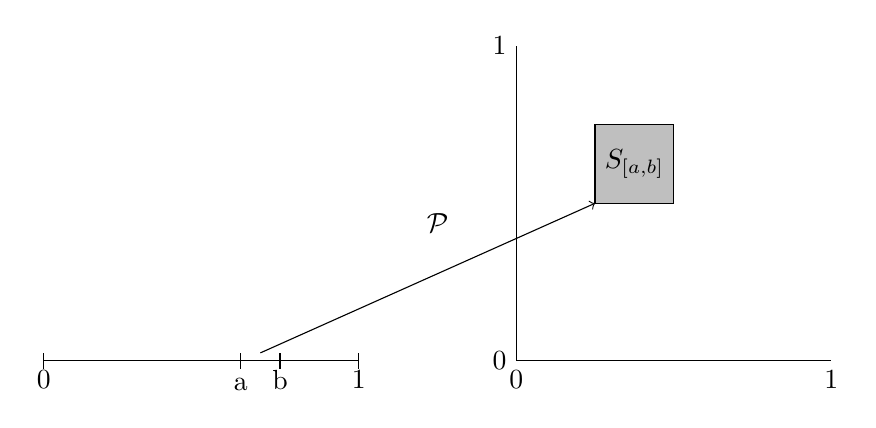
\begin{tikzpicture}
\draw (0,0) -- (4,0);
\tick{0};
\tick{2.5};
\tick{3};
\tick{4};
\node [below] at (0,0) {0};
\node [below] at (2.5,-0.1) {a};
\node [below] at (3,0) {b};
\node [below] at (4,0) {1};

\draw (6,0) -- (10,0);
\draw (6,0) -- (6,4);
\node [below] at (6,0) {0};
\node [left] at (6,0) {0};
\node [below] at (10,0) {1};
\node [left] at (6,4) {1};
\draw [fill=lightgray] (7,2) rectangle (8,3);
\node at (7.5,2.5) {$S_{[a,b]}$};
\draw [->] (2.75, 0.1) -- (7,2);
\node at (5,1.75) {$\pc$};
\end{tikzpicture}

Such a mapping is called a \emph{Peano Mapping} and its corresponding curve is
called a \emph{Peano Curve}.

Note that this is a parameterized curve from domain $\mathbb{R}$ to co-domain
$\mathbb{R}^2$. It is not a mapping \emph{on} $\mathbb{R}$ and thus is not
subject to our normal intuitive notions of a curve in $\mathbb{R}^2$.

\newpage

\section*{Quartic Intervals}

Start with $\uint$ and with each generation, subdivide each sub-interval
into four equal parts.  Designate each sub-interval as $I_k^n$, where $n$ is
the generation and $k$ is the relative position of the interval (starting
from 0).

\begin{tikzpicture}
\node at (-1,0) {\large$I^0$:};
\draw (0,0) -- (8,0);
\tick{0};
\tick{8};
\node [below] at (0,0) {\small0};
\node [below] at (8,0) {\small1};
\node [below] at (4,-0.5) {\small$I_0^0$};
\end{tikzpicture}

\begin{tikzpicture}
\node at (-1,0) {\large$I^1$:};
\draw (0,0) -- (8,0);
\tick{0};
\tick{2};
\tick{4};
\tick{6};
\tick{8};
\node [below] at (0,0) {\small0};
\node [below] at (2,0) {\small$\frac{1}{4}$};
\node [below] at (4,0) {\small$\frac{2}{4}$};
\node [below] at (6,0) {\small$\frac{3}{4}$};
\node [below] at (8,0) {\small1};
\node [below] at (1,-0.5) {\small$I_0^1$};
\node [below] at (3,-0.5) {\small$I_1^1$};
\node [below] at (5,-0.5) {\small$I_2^1$};
\node [below] at (7,-0.5) {\small$I_3^1$};
\end{tikzpicture}

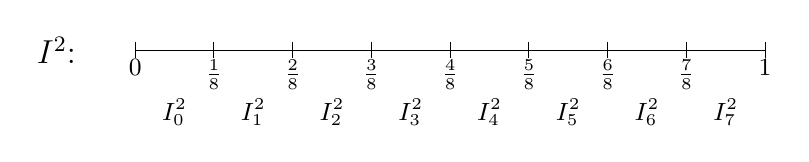
\begin{tikzpicture}
\node at (-1,0) {\large$I^2$:};
\draw (0,0) -- (8,0);
\tick{0};
\tick{1};
\tick{2};
\tick{3};
\tick{4};
\tick{5};
\tick{6};
\tick{7};
\tick{8};
\node [below] at (0,0) {\small0};
\node [below] at (1,0) {\small$\frac{1}{8}$};
\node [below] at (2,0) {\small$\frac{2}{8}$};
\node [below] at (3,0) {\small$\frac{3}{8}$};
\node [below] at (4,0) {\small$\frac{4}{8}$};
\node [below] at (5,0) {\small$\frac{5}{8}$};
\node [below] at (6,0) {\small$\frac{6}{8}$};
\node [below] at (7,0) {\small$\frac{7}{8}$};
\node [below] at (8,0) {\small1};
\node [below] at (1/2,-0.5) {\small$I_0^2$};
\node [below] at (3/2,-0.5) {\small$I_1^2$};
\node [below] at (5/2,-0.5) {\small$I_2^2$};
\node [below] at (7/2,-0.5) {\small$I_3^2$};
\node [below] at (9/2,-0.5) {\small$I_4^2$};
\node [below] at (11/2,-0.5) {\small$I_5^2$};
\node [below] at (13/2,-0.5) {\small$I_6^2$};
\node [below] at (15/2,-0.5) {\small$I_7^2$};
\end{tikzpicture}

\begin{tikzpicture}
\node at (-1,0) {\large$I^n$:};
\draw (0,0) -- (8,0);
\tick{0};
\tick{3};
\tick{4};
\tick{8};
\node [below] at (0,0) {\small0};
\node [below] at (1.5,0) {\small\ldots};
\node [below] at (3,0) {\small$\frac{k}{4^n}$};
\node [below] at (4,0) {\small$\frac{k+1}{4^n}$};
\node [below] at (6,0) {\small\ldots};
\node [below] at (8,0) {\small1};
\node [below] at (7/2,-0.5) {\small$I_k^n$};
\end{tikzpicture}

Each generation has $4^n$ intervals of length
(measure):\ $m_1(I_k^n)=\frac{1}{4^n}$.

\begin{definition}
A \emph{chain} of quartic intervals is a decreasing sequence:
\[I^0\subset I^1\subset I^2\subset\ldots\subset I^k\subset\ldots\]
where $I^k$ is a quartic interval of the $k^{th}$ generation.
\end{definition}

\begin{properties}
\listbreak
\begin{enumerate}
\item If $(I^k)$ is a chain of quartic intervals then there exists a unique
$t\in\uint$ such that $t\in\bigcap_kI^k$.

\item Conversely, given $t\in\uint$, there is a chain $(I^k)$ of quartic
intervals such that $t\in\bigcap_kI^k$.

\item The set of $t$ for which the chain in $(ii)$ is not unique is a countable
set of measure 0.
\end{enumerate}
\end{properties}

Note that the non-uniqueness occurs at the boundaries of each quartic interval,
at the points $\{\frac{j}{4^k}|0<j<4^k\}$, the set of \emph{dyadic rationals},
which is countable and has measure 0.

Similar to the Cantor-Lebesgue function, we can represent each chain with
a base-4 string of the form $0.a_1a_2\cdots a_k\cdots$ where each digit
selects one of the 4 sub-intervals in an interval from the previous generation.
Thus, each $t\in\uint$ can be expressed as:
\[t=\sum_{k=1}^{\infty}\frac{a_k}{4^k}\]
which is well-defined except at the dyadic rationals, which correspond to
numbers of the form:
\[0.a_1a_2\cdots a_k0000\cdots=0.a_1a_2\cdots (a_k-1)3333\cdots\]
on the interval boundaries.

\newpage

\subsection*{Dyadic Squares}

Start with $\usq$ and with each generation, subdivide each sub-square
into four equal parts.  Designate each sub-interval as $I_{r,c},^n$, where $n$ is
the generation, $r$ is the row, and $c$ is the column.  Row and column
numbering starts from 0, with $(0,0)$ being in the lower left-hand corner.

\begin{tikzpicture}
\node at (-2,2) {\large$S^0$:};
\draw (0,0) -- (4,0);
\draw (0,4) -- (4,4);
\draw (0,0) -- (0,4);
\draw (4,0) -- (4,4);
\node [below] at (0,0) {\small0};
\node [below] at (4,0) {\small1};
\node [left] at (0,0) {\small0};
\node [left] at (0,4) {\small1};
\node at (2,2) {\small$S_{0,0}^0$};
\end{tikzpicture}
\hspace{0.5in}
\begin{tikzpicture}
\node at (-2,2) {\large$S^1$:};
\draw (0,0) -- (4,0);
\draw (0,2) -- (4,2);
\draw (0,4) -- (4,4);
\draw (0,0) -- (0,4);
\draw (2,0) -- (2,4);
\draw (4,0) -- (4,4);
\node [below] at (0,0) {\small0};
\node [below] at (2,0) {\small$\frac{1}{2}$};
\node [below] at (4,0) {\small1};
\node [left] at (0,0) {\small0};
\node [left] at (0,2) {\small$\frac{1}{2}$};
\node [left] at (0,4) {\small1};
\node at (1,1) {\small$S_{0,0}^1$};
\node at (3,1) {\small$S_{0,1}^1$};
\node at (1,3) {\small$S_{1,0}^1$};
\node at (3,3) {\small$S_{1,1}^1$};
\end{tikzpicture}

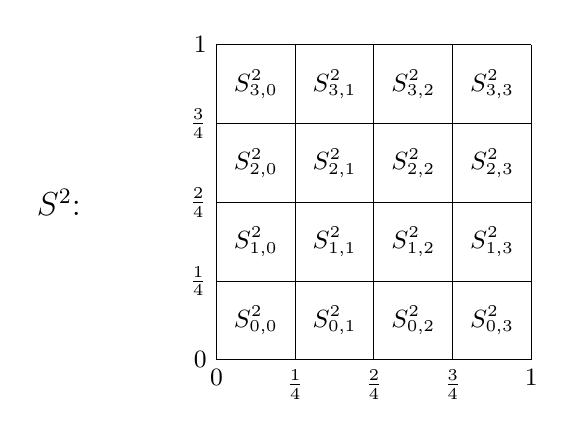
\begin{tikzpicture}
\node at (-2,2) {\large$S^2$:};
\draw (0,0) -- (4,0);
\draw (0,1) -- (4,1);
\draw (0,2) -- (4,2);
\draw (0,3) -- (4,3);
\draw (0,4) -- (4,4);
\draw (0,0) -- (0,4);
\draw (1,0) -- (1,4);
\draw (2,0) -- (2,4);
\draw (3,0) -- (3,4);
\draw (4,0) -- (4,4);
\node [below] at (0,0) {\small0};
\node [below] at (1,0) {\small$\frac{1}{4}$};
\node [below] at (2,0) {\small$\frac{2}{4}$};
\node [below] at (3,0) {\small$\frac{3}{4}$};
\node [below] at (4,0) {\small1};
\node [left] at (0,0) {\small0};
\node [left] at (0,1) {\small$\frac{1}{4}$};
\node [left] at (0,2) {\small$\frac{2}{4}$};
\node [left] at (0,3) {\small$\frac{3}{4}$};
\node [left] at (0,4) {\small1};
\node at (1/2,1/2) {\small$S_{0,0}^2$};
\node at (3/2,1/2) {\small$S_{0,1}^2$};
\node at (5/2,1/2) {\small$S_{0,2}^2$};
\node at (7/2,1/2) {\small$S_{0,3}^2$};
\node at (1/2,3/2) {\small$S_{1,0}^2$};
\node at (3/2,3/2) {\small$S_{1,1}^2$};
\node at (5/2,3/2) {\small$S_{1,2}^2$};
\node at (7/2,3/2) {\small$S_{1,3}^2$};
\node at (1/2,5/2) {\small$S_{2,0}^2$};
\node at (3/2,5/2) {\small$S_{2,1}^2$};
\node at (5/2,5/2) {\small$S_{2,2}^2$};
\node at (7/2,5/2) {\small$S_{2,3}^2$};
\node at (1/2,7/2) {\small$S_{3,0}^2$};
\node at (3/2,7/2) {\small$S_{3,1}^2$};
\node at (5/2,7/2) {\small$S_{3,2}^2$};
\node at (7/2,7/2) {\small$S_{3,3}^2$};
\end{tikzpicture}
\hspace{0.5in}
\begin{tikzpicture}
\node at (-2,2) {\large$S^n$:};
\draw (0,0) rectangle (4,4);
\draw (1,2) rectangle (2,3);
\draw [dashed] (1,0) -- (1,2);
\draw [dashed] (2,0) -- (2,2);
\draw [dashed] (0,2) -- (1,2);
\draw [dashed] (0,3) -- (1,3);
\node [below] at (0,0) {\small0};
\node [below] at (1,0) {\small$\frac{c}{2^n}$};
\node [below] at (2,0) {\small$\frac{c+1}{2^2}$};
\node [below] at (4,0) {\small1};
\node [left] at (0,0) {\small0};
\node [left] at (0,2) {\small$\frac{r}{2^n}$};
\node [left] at (0,3) {\small$\frac{r+1}{2^n}$};
\node [left] at (0,4) {\small1};
\node at (3/2,5/2) {\small$S_{r,c}^n$};
\end{tikzpicture}

Each generation has $4^n$ squares ($2^n\times2^n$) of area
(measure):\ $m_2(S_{r,c}^n)=\frac{1}{4^n}$.

\begin{definition}
A \emph{chain} of dyadic squares is a decreasing sequence:
\[S^0\subset S^1\subset S^2\subset\ldots\subset S^k\subset\ldots\]
where $S^k$ is a dyadic square of the $k^{th}$ generation.
\end{definition}

\begin{properties}
\listbreak
\begin{enumerate}
\item If $(S^k)$ is a chain of dyadic squares then there exists a unique
$x\in\usq$ such that $x\in\bigcap_kS^k$.

\item Conversely, given $x\in\usq$, there is a chain $(S^k)$ of dyadic
squares such that $x\in\bigcap_kS^k$.

\item The set of $x$ for which the chain in $(ii)$ is not unique is a countable
set of measure 0.
\end{enumerate}
\end{properties}

Note that the non-uniqueness occurs at all points $(x_1,x_2)$, where at least
one of the coordinates is a dyadic rational ($4^k=2^{2k}$), corresponding to the
countable set of vertical and horizontal line sequences of measure 0.

Similar to the Cantor-Lebesgue function, we can represent each chain
with a base-4 string of the form $0.b_1b_2\cdots b_k\cdots$ where each digit
selects one of the 4 sub-squares in a square from the previous generation.
Thus, each $x\in\usq$ can be expressed as:
\[x=\sum_{k=1}^{\infty}\frac{\overline{b}_k}{4^k}\]
where
\[\overline{b}_k=\left\{\begin{array}{ll}
(0,0) & b_k=0 \\
(0,1) & b_k=1 \\
(1,0) & b_k=2 \\
(1,1) & b_k=3\end{array}
\right.\]

\newpage

\subsection*{Dyadic Correspondence}

Note that: $|I^n|=|S^n|$ and $m_1(I_k^n)=m_2(S_{r,c}^n)$. So, we would like to
establish a bijection between the intervals in the domain and the squares in
the co-domain.

\begin{definition}
A \emph{dyadic correspondence} is a mapping $\Phi$ from quartic intervals to
dyadic squares such that:
\begin{enumerate}
\item $\Phi$ is bijective.
\item $\Phi$ respects generations: $I\in I^k\implies\Phi(I)\in S^k$.
\item $\Phi$ respects inclusion: $I\subset J\implies\Phi(I)\subset\Phi(J)$.
\end{enumerate}
\end{definition}

The trivial correspondence is given by $a_k=b_k$ in the base-4 representations
of each chain; however, this results in a discontinuous mapping of intervals
to rectangles.

We can now define the \emph{induced mapping} $\Phi^*:\uint\to\usq$. Let
$\{t\}=\bigcap_{k=1}^{\infty}I^k$ where $(I^k)$ is a chain of quartic intervals.
Then, by definition, $(\Phi(I^k))$ is a chain of dyadic squares such that
$\bigcap_{k=1}^{\infty}\Phi(I^k)=\{x\}$ and:
\[\Phi^*(t)=x\]

Note that if $I$ is a quartic interval of the $k^{th}$ generation then
$\Phi^*[I]=\Phi(I)$, where $\Phi(I)$ is a dyadic square of the $k^{th}$
generation and: $m_1(I)=m_2(\Phi^*[I])$.

The problem with $\Phi^*$ is that it is not well-defined on the interval
boundary points, since each is representable by two different quartic chains,
resulting in two different dyadic chains.

\newpage

\section*{Key Theorem}

\begin{theorem}
Given a dyadic correspondence $\Phi$, there exists sets $Z_1\subset\uint$ and
$Z_2\subset\usq$, both of measure 0, such that:
\begin{enumerate}
\item $\Phi^*:\uint-Z_1\to\usq-Z_2$ is a bijection.
\item $E\subset\uint$ is measurable iff $\Phi^*[E]$ is measurable.
\item $m_1(E)=m_2(\Phi^*[E])$.
\end{enumerate}
\end{theorem}

First part follows by excluding all points that do not have unique chains.

The fact that these points form a set of measure 0 follows from the lemma that
if $a_k$ differs from some fixed $f_k$ for $k$ sufficiently large then the
resulting set has measure 0.

Last part is a repeat of Theorem 1.4, only this time use dyadic squares for
the covering of the open subset of $\mathbb{R}^2$.

\newpage

\section*{Traversal}

Given a dyadic square $S$ in generation $k$, consider its four sub-squares in
generation $k+1$. Assuming we can enter at any square $S_1$, we can always
traverse adjacent squares in a sequence $(S_1, S_2, S_3, S_4)$ and exit at any
edge $\sigma$.  The four possibilities are:

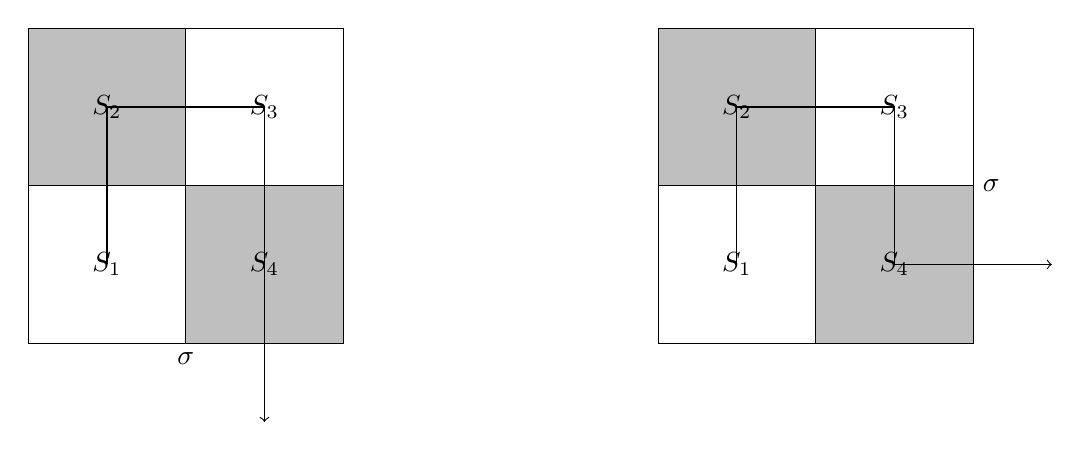
\begin{tikzpicture}
\draw (0,0) rectangle (2,2);
\draw [fill=lightgray] (0,2) rectangle (2,4);
\draw (2,2) rectangle (4,4);
\draw [fill=lightgray] (2,0) rectangle (4,2);
\node at (1,1) {$S_1$};
\node at (1,3) {$S_2$};
\node at (3,3) {$S_3$};
\node at (3,1) {$S_4$};
\node [below] at (2,0) {$\sigma$};
\draw [->] (1,1) -- (1,3) -- (3,3) -- (3,1) -- (3,-1);

\draw (8,0) rectangle (10,2);
\draw [fill=lightgray] (8,2) rectangle (10,4);
\draw (10,2) rectangle (12,4);
\draw [fill=lightgray] (10,0) rectangle (12,2);
\node at (9,1) {$S_1$};
\node at (9,3) {$S_2$};
\node at (11,3) {$S_3$};
\node at (11,1) {$S_4$};
\node [right] at (12,2) {$\sigma$};
\draw [->] (9,1) -- (9,3) -- (11,3) -- (11,1) -- (13,1);
\end{tikzpicture}

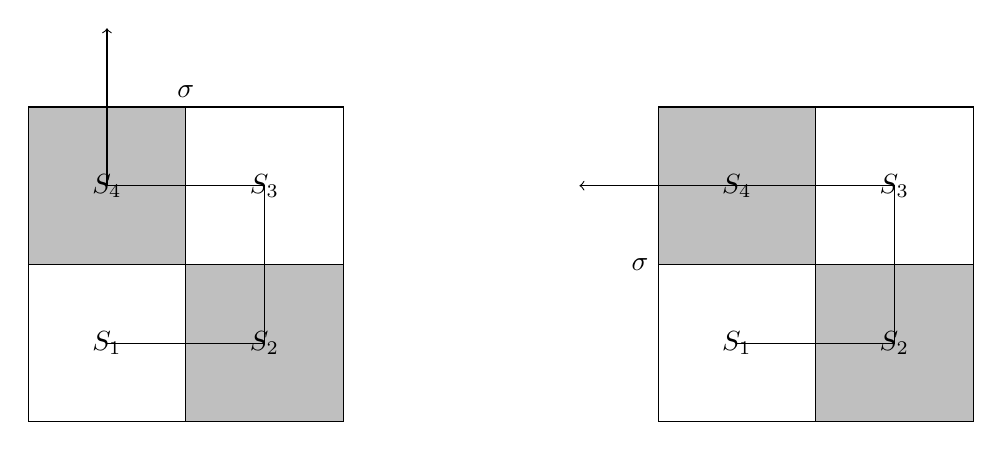
\begin{tikzpicture}
\draw (0,0) rectangle (2,2);
\draw [fill=lightgray] (0,2) rectangle (2,4);
\draw (2,2) rectangle (4,4);
\draw [fill=lightgray] (2,0) rectangle (4,2);
\node at (1,1) {$S_1$};
\node at (1,3) {$S_4$};
\node at (3,3) {$S_3$};
\node at (3,1) {$S_2$};
\node [above] at (2,4) {$\sigma$};
\draw [->] (1,1) -- (3,1) -- (3,3) -- (1,3) -- (1,5);

\draw (8,0) rectangle (10,2);
\draw [fill=lightgray] (8,2) rectangle (10,4);
\draw (10,2) rectangle (12,4);
\draw [fill=lightgray] (10,0) rectangle (12,2);
\node at (9,1) {$S_1$};
\node at (9,3) {$S_4$};
\node at (11,3) {$S_3$};
\node at (11,1) {$S_2$};
\node [left] at (8,2) {$\sigma$};
\draw [->] (9,1) -- (11,1) -- (11,3) -- (9,3) -- (7,3);
\end{tikzpicture}

Note that each entry square is colored white and each exit square is colored
black.

\newpage

\section*{Dyadic Correspondence with Adjacency}

\begin{theorem}
There exists a dyadic correspondence $\Phi$ such that:
\begin{enumerate}
\item In generation $k$, Let $I_{-}$ be the leftmost interval and $I_{+}$ be the
rightmost interval.  $\Phi(I_{-})$ is the lower left square and $\Phi(I_{+})$ is
the lower right square.

\item If $I$ and $J$ are two adjacent intervals in generation $k$ then
$\Phi(I)$ and $\Phi(J)$ are adjacent squares in generation $k$.
\end{enumerate}
\end{theorem}

\begin{theproof}[by Induction on $k$]
\listbreak
\begin{description}

\item{Base:} $k=1$

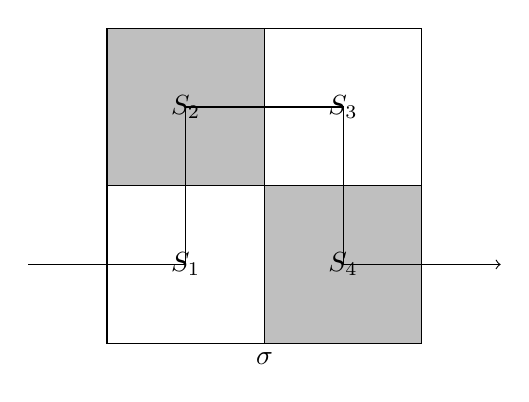
\begin{tikzpicture}
\draw (0,0) rectangle (2,2);
\draw [fill=lightgray] (0,2) rectangle (2,4);
\draw (2,2) rectangle (4,4);
\draw [fill=lightgray] (2,0) rectangle (4,2);
\node at (1,1) {$S_1$};
\node at (1,3) {$S_2$};
\node at (3,3) {$S_3$};
\node at (3,1) {$S_4$};
\node [below] at (2,0) {$\sigma$};
\draw [->] (-1,1) -- (1,1) -- (1,3) -- (3,3) -- (3,1) -- (5,1);
\end{tikzpicture}

\item{Assume $\Phi$ has been defined for all generations $\le k$}

\item{Consider generation $k+1$}

Assume that $S_j$ is a square from generation $k$ that has been divided into
squares $S_{j,1}, S_{j,2}, S_{j,3}, S_{j,4}$ in generation $k+1$. \\
Square $S_j$ is entered from adjacent square $S_{j-1}$ by a traversal from a
black square in $S_{j-1}$ to a white square in $S_j$. \\
Let $\sigma$ be the edge between $S_j$ and $S_{j+1}$. \\
Traverse $S_j$ using one of the four valid traversals to reach $S_{j+1}$. \\
By the inductive assumption $S_{4^k}$ is in the lower-right corner, and must be
entered from adjacent square $S_{4^k-1}$ from either the top or left. \\
Since the lower left square in generation $k+1$ is an exit square, it must be
black. Since we must enter $S_{4^k}$ on a white square, only one of the
following two cases is possible:

\newpage

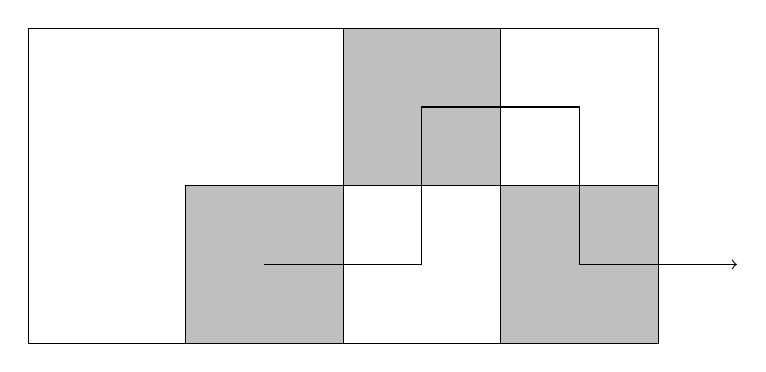
\begin{tikzpicture}
\draw (0,0) rectangle (4,4);
\draw [fill=lightgray] (2,0) rectangle (4,2);
\draw (4,0) rectangle (6,2);
\draw [fill=lightgray] (4,2) rectangle (6,4);
\draw (6,2) rectangle (8,4);
\draw [fill=lightgray] (6,0) rectangle (8,2);
\draw [->] (3,1) -- (5,1) -- (5,3) -- (7,3) -- (7,1) -- (9,1);
\end{tikzpicture}

\vspace{0.5in}

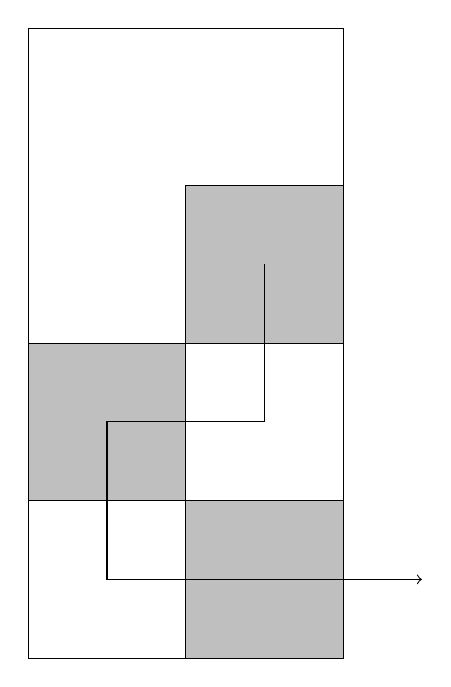
\begin{tikzpicture}
\draw (0,0) rectangle (2,2);
\draw [fill=lightgray] (0,2) rectangle (2,4);
\draw (2,2) rectangle (4,4);
\draw [fill=lightgray] (2,0) rectangle (4,2);
\draw (0,4) rectangle (4,8);
\draw [fill=lightgray] (2,4) rectangle (4,6);
\draw [->] (3,5) -- (3,3) -- (1,3) -- (1,1) -- (3,1) -- (5,1);
\end{tikzpicture}

\vspace{0.5in}

$\therefore$, $\Phi$ is properly defined for generation $k+1$.

\end{description}
\end{theproof}

\newpage

\section*{The Curve}

Let $\Phi$ be the dyadic correspondence described above. For generation $k$,
let $t_j$ be the center of the $j^{th}$ quartic interval:
\[t_j=\frac{j-\frac{1}{2}}{4^k}, 1\le j\le4^k\]
and let $x_j$ be the center of the $j^{th}$ square per the ordering imposed by
$\Phi$. Define:
\[\pc(t)=\left\{\begin{array}{ll}
x_j & t=t_j \\
(0,\frac{1}{2^{k+1}})=x_0 & t=t_0=0 \\
(1,\frac{1}{2^{k+1}})=x_{4^k+1} & t=t_{4^k+1}=1 \\
\end{array}\right.\]
Then linearly extend the values between the $t_j$ to create a set of horizontal
and vertical lines between the centers.

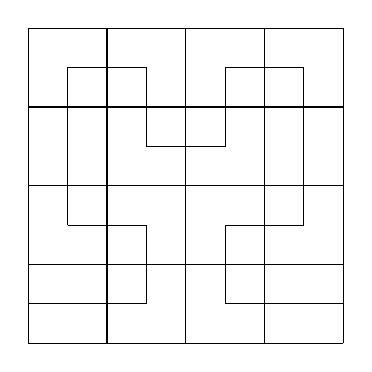
\begin{tikzpicture}
\draw (0,0) -- (4,0);
\draw (0,1) -- (4,1);
\draw (0,2) -- (4,2);
\draw (0,3) -- (4,3);
\draw (0,4) -- (4,4);
\draw (0,0) -- (0,4);
\draw (1,0) -- (1,4);
\draw (2,0) -- (2,4);
\draw (3,0) -- (3,4);
\draw (4,0) -- (4,4);
\draw (0,1/2) -- (3/2,1/2) -- (3/2,3/2) -- (1/2,3/2);
\draw (1/2,3/2) -- (1/2,7/2) -- (3/2,7/2) -- (3/2,5/2);
\draw (1/2,3/2) -- (1/2,7/2) -- (3/2,7/2) -- (3/2,5/2);
\draw (3/2,5/2) -- (5/2,5/2) -- (5/2,7/2) -- (7/2,7/2);
\draw (7/2,7/2) -- (7/2,3/2) -- (5/2,3/2) -- (5/2,1/2) -- (4,1/2);
\end{tikzpicture}

\begin{theorem}
$P_k(t)$ is continuous.
\end{theorem}

\begin{theproof}
Assume $\epsilon>0$ \\
Let $\delta=min\{\frac{1}{4^k}, \frac{\epsilon}{2^k}\}$ \\
Along each line segment, $P_k'(t)=\frac{\frac{1}{2^k}}{\frac{1}{4^k}}=2^k$ \\
Assume $|t_i-t_j|<\delta$ \\
\begin{description}

\item{case 1: $\delta=\frac{1}{4^k}$}
\[|\pc(t_i)-\pc(t_j)|\le\frac{1}{2^k}<\epsilon\]

\item{case 2: $\delta=\frac{\epsilon}{2^k}$}
\[|\pc(t_i)-\pc(t_j)|\le2^k|t_i-t_j|<2^k(\frac{\epsilon}{2^k})=\epsilon\]

\end{description}
\end{theproof}

\begin{theorem}
$\pc$ exists, is continuous, and is onto (surjective).
\end{theorem}

\begin{theproof}
Assume $t\in\uint$ \\
Assume $\epsilon>0$ \\
Let $N(\epsilon)=\log_2\frac{\sqrt{2}}{\epsilon}$ \\
Assume $k>N$ \\
\[|\pc_{k+1}(t)-\pc_k(t)|\le\frac{\sqrt{2}}{2^k}<
    \frac{\sqrt{2}}{2^{\log_2\frac{\sqrt{2}}{\epsilon}}}=\epsilon\]
The continuous $\pc_k$ converge uniformly to some $\pc$, which is also
continuous. \\
But $\pc$ is also dense in $\usq$ and is thus onto as well.
\end{theproof}

\begin{theorem}
Let $\Phi$ be the dyadic correspondence from above. $\Phi^*(t)=\pc(t)$.
\end{theorem}

\begin{theproof}
Assume $[a,b]\in\uint$ \\
$(a,b)$ can be written as $\bigcup_jI_j$, where the $I_j$ are quartic intervals
with disjoint interiors. \\
\[m_2(\pc(a,b))=\sum_{j=1}^{\infty}m_2(\pc(I_j))=\sum_{j=1}^{\infty}m_1(I_j)=m_1(a,b)\]
\end{theproof}

\end{document}
